In this section, we provide background on SoC platforms, timing side-channels and non-interference properties.

\subsection{SoC platforms}

\begin{figure}[t]
    \begin{center}
    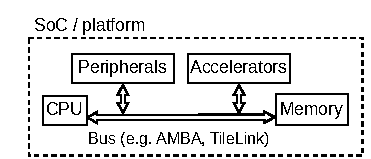
\includegraphics[width=0.8\columnwidth]{figures/exampleplatform/exampleplatform.pdf}
    \end{center}
    \vspace*{-1em}
    \caption{\label{fig:exampleplatform}
        Example SoC platform architecture.
    }
    \vspace*{-1em}
\end{figure}

In this paper, we use the words SoC, system and platform interchangeably to refer to the integrated circuit that integrates various components, including CPUs, memory, and peripherals, as illustrated in Fig.~\ref{fig:exampleplatform}.
The communication between these components is typically managed through standardized bus protocols, such as AMBA~\cite{arm_amba} or TileLink~\cite{tilelink_spec}.
The bounds of components are not always clear-cut.
For example, Fig.~\ref{fig:verifscopecache} shows that caches can be considered part of the CPU or of the rest of the platform.
For a hardware component, we refer to its \emph{input signals} as the inbound wires, and its \emph{inputs} as the values carried by those wires, and similarly for outputs.

\subsection{Timing side-channels}

Multiple hardware optimizations, such as caches and branch predictors, learn and exploit patterns in program execution to improve performance.
In particular, the execution time of later instructions may depend on the outcome of earlier instructions.
For example, accessing a cache line might be faster if the line has been brought into the cache recently by a prior memory access to a nearby location.
% Timing side channels can result from such optimizations when the timing of a program's execution depends on secret data.
Constant-time programming techniques, such as not using secret data as array indices or loop conditions, aim to ensure that secrets do not influence the execution time of a program through such channels~\cite{OsvikShamirTromer2006CacheAES,AlmeidaEtAl2016CTVerif}.

\subsection{Information Flow Tracking}
\label{subsec:ift}

\begin{figure}[t]
    \begin{center}
    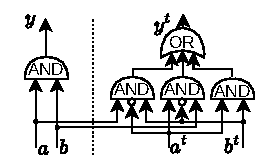
\includegraphics[width=0.5\columnwidth]{figures/glift/glift.pdf}
    \end{center}
    \vspace*{-1em}
    \caption{\label{fig:glift} Taint tracking at gate level~\cite{tiwari2009complete}. Left: original circuit. Right: Added instrumentation for taint tracking. The original input signals are $a$ and $b$. The taint bits corresponding to $a$ and $b$ are respectively $a^t$ and $b^t$. The output taint bit $y^t$ indicates whether the output is tainted, i.e., influenced by the tainted inputs.}
    \vspace*{-1em}
\end{figure}

\begin{figure}[t]
    \begin{center}
    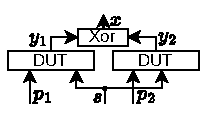
\includegraphics[width=0.5\columnwidth]{figures/miter/miter.pdf}
    \end{center}
    \vspace*{-2em}
    \caption{\label{fig:miter} Miter circuit. The two instances of the same DUT are supplied with the same public data $p$ and unconstrained $s_1$ and $s_2$ secret data. The output bit $y$ (i.e., instantiated for the instances in the miter as $y_1$ and $y_2$) reveals secret data if $x=1$ is satisfiable.}
    % \vspace*{-1em}
\end{figure}

Hardware information flows capture properties such as confidentiality and integrity~\cite{hu2021hardware}.
They are typically tracked using one of two techniques.
The first technique is called dynamic information flow tracking (DIFT).
It captures information flows by augmenting the hardware design under test (DUT) with a synthesizable instrumentation that computes the propagation of taint bits~\cite{tiwari2009complete,ardeshiricham2017register,solt2022cellift,solt2024hybridift,ceesay2024mucfi} as shown in Fig.~\ref{fig:glift}.
The second technique is called a miter circuit.
It captures information flows by comparing the outputs of two copies of the DUT, where all inputs except the sources are unconstrained, while all the others are equal as illustrated in Fig.~\ref{fig:miter}.

\subsection{Hardware-software contracts}
\label{subsec:hw-sw-contracts}

\para{Contract definition}
Hardware-software contracts~\cite{guarnieri2021hardware} split confidentiality responsibilities between the CPU and the software that it executes.
For an initial microarchitectural state, a given program $P$, and the contents of memory containing public information $M_p$ and secret information $M_s$, the contract specifies an execution mode and an observation mode.
The \emph{execution mode} determines which instructions are executed (potentially transiently) and generate events.
The \emph{observation mode} determines which of those events are exposed to an observer (possibly transiently), such as the addresses or values involved in memory accesses.
Under such a contract, the CPU's behavior is summarized as a sequence of observable events known as a hardware trace~\cite{guarnieri2021hardware,oleksenko2022revizor}.

\para{Contract verification}
Multiple independent verification efforts have been conducted to ensure that hardware-software contracts are upheld during program execution, in particular regarding constant-time behavior~\cite{dinesh2024conjunct,ceesay2024mucfi,guarnieri2021hardware,tan2025contractshadowlogic,dinesh2025h,hsiao2024rtl2mmupath,wang2023specification}.
Most techniques consider a fixed contract~\cite{dinesh2024conjunct,ceesay2024mucfi,tan2025contractshadowlogic,dinesh2025h}, while some others leverage custom, non-trivial technique-specific insights to verify a wider variety of contracts~\cite{hsiao2024rtl2mmupath,wang2023specification} using the same technique.

\para{Discussion}
These techniques make assumptions about the platform in which the CPU is integrated, yet there exists no language for formally expressing and verifying them.
